%  \documentclass[letter]{IEEEtran}
  \documentclass[letter]{article}
\usepackage[utf8]{inputenc}
%\usepackage[margin=1in]{geometry}
\usepackage{tikz}
\usepackage{ulem}
\usepackage{graphics}
\usepackage{sidecap}
\usepackage{wrapfig}
\usepackage[toc,page]{appendix}
\usepackage{caption}
\usepackage{subcaption}

\usepackage{hyperref}
\hypersetup{
    colorlinks,%
    citecolor=black,%
    filecolor=black,%
    linkcolor=black,%
    urlcolor=black
}

\def\dashuline{\bgroup 
  \ifdim\ULdepth=\maxdimen  % Set depth based on font, if not set already
	  \settodepth\ULdepth{(j}\advance\ULdepth.4pt\fi
  \markoverwith{\kern.15em
	\vtop{\kern\ULdepth \hrule width .3em}%
	\kern.15em}\ULon}

\newcounter{foot}
\setcounter{foot}{1}

\author{Christopher Patton}
\date{\today}
\title{Salamander: computer vision for wildlife research}
	
\begin{document}
\maketitle

\begin{abstract}
This document outlines an image prcessing application called Salamander. Salamander
is comprised of a set of algorithms for automatically detecting and tracking 
targets of interest in a video stream. It is particularly useful for filtering 
and segmenting video produced by field cameras for wildlife and behaviorial 
research. 
\end{abstract}

\tableofcontents
\pagebreak 

\section{Introduction}
[TODO] Overview of approach. Define each task: detection, tracking, and segmentaiton. 

\section{Algorithms}
I now describe our approach to target detection and tracking and segmentation of 
the video stream. We make the following basic assumptions about the video and our
targets:  
\begin{enumerate}
  \item The camera is fixed. 
  
  \item The rate at which pictures are taken is fixed.\footnote{It may be necessary
   in certain implementations to covercome this assumption. For example, a field 
   camera may transmit its video stream over a network. The rate at which pictures 
   are taken can be set to depend on network conditions. However, It is possible to 
   assume a lowest-possible rate and tune Salamander accordingly.}

  \item The targets are the same species, i.e., roughly the sames size and color. 
   Under typical circumstances, its not practical to look for deer and mice 
   simultaneously.
  
  \item Targets are roughly the same distance away from the camera when we detect them. 
   
\end{enumerate}

The reasons for these assumptions will become apparent in this section. They are 
necessary for the basic functionality of the algorithms we'll describe, but it may
be possible to disregard at (3) and (4) with machine learning. We'll explore this 
possibility in section 3. However, we must assume (1) in any case. 

Initial image processing, detection, tracking, and segmentation are layered. By this 
we mean that in order to achieve one task, all preceeding tasks must be accomplished first. 
We describe each layer and the corresponding algorithms and data structures in turn. 
In the following sections, a video stream is represented by a sequence of video frames:
$$ \langle v_0, v_1, v_2, \dots v_{n-1}, v_n \rangle $$

\subsection{Image processing}
The first step in our approach is to calculate the pixelwise difference of two
adjacent frames in a video stream. The resulting image, which we'll refer to as
the \textit{delta} image, tells us which regions of the image changed within that 
unit of time. We'll perfom some additional filtering, then search the image for 
\textit{blobs}, contiguous regions of \textit{delta} that correspond to significant 
changes. At this point, image processing is finished and we can proceed to detection. 


 \textbf{delta} $\delta(v_{i-1}, v_i) \rightarrow d_i$. Input images are typically JPEG 
format. Each pixel of a JPEG image is represented by three bytes corresponding 
to the red, blue, and green luminance. To simplify the following steps of the 
pipeline, we first convert $v_{i-1}$ and $v_i$ to gray scale images with floating point 
precision. Next we subtract 
$v_{i}$ from $v_{i-1}$ and store the absolute value of each pixel. Now, all changes in 
the frame within the time points $i-1$ to $i$ are reflected in the delta image $d_i$. 
We can analyse these changes in order to determine if a target has appeared in frame.


 
 \textbf{binary threshold} $b(d_i) \rightarrow b_i$. The next step converts all pixels 
to one of two values \{white, black\}, which is needed for subsequent filters. 
This step also allows us to deal with noise artifacts related to the quality of the 
image taken, e.g. bluriness, compressing and decompressing JPEGs, gray scale 
filtering, etc.[\textbf{ref}] More to the point, if a pixel has changed just a little, we set it to 
black; if it's changed a lot, we set it to white. For each pixel $p$ in $d_i$ and 
threshold range $l$ and $h$ where $l < h$, 
\[
 b_i(p) = \left \{
  \begin{array}{ll}
    \textrm{white} & l \le d_i(p) \le h \\
    \textrm{black} & \textrm{otherwise.}
  \end{array} \right.
\] 

 \textbf{binary morphology} $m(b_i) \rightarrow m_i$. finally, the last filter 
enables us to deal with physical noise. This includes things like shadows,
small objects such as leaves or grass being blown around by the wind, and small
insects we may not care about. Morphology has two stages: in erosion, the edges of
artifacts in $b_i$ are worn away iteratively. Small noise artifacts will disappear 
as a result, leaving only those that correspond to actual targets; in dilation, we 
inflate the remaining blobs by doing the reverse of erosion. We iteratively add layers
to the surfaces of remaining blobs. 
Typically, many more dilation as erosion rounds are used, so that artifacts that 
comprise a single target, i.e., those that are near to each other, will merge together.
Binary morphology is the most computationally expensive stage of the image processing
pipeline. Once we're done, we're ready to analyse the remaining \textit{blobs} for 
the presence of targets. 

  \textbf{connected component analysis} $c(m_i) \rightarrow \textit{Blob list}$. 
The final image processing step allows us to disvoer the locations of blobs in 
$m_i$ and provides some useful information about them. The connected component analysis
algorithm, analogous to its counter-part graph theory, returns a list of connected 
regions in the image. In the binary image $m_i$, this is simply contiguous regions
of the same color. The black background is one such region; the rest are the blobs
remaining after binary morphology. Let $c(m_i): \rightarrow \textit{Blob list}$ be a 
function that performs this analysis and returns a list of blobs with the following attributes: 
\[
 \textit{Blob} = \left (
  \begin{array}{ll}
    \textit{bbox} (l,r,t,b) \texttt{ int} & \textrm{Rectangular region bounding the blob.} \\
    \textit{centr} (x, y) \texttt{ int} &   \textrm{Coordinates of blob centroid.} \\ 
    \textit{vol} \texttt{ int} &            \textrm{The number of pixels that comprise the blob.} \\
  \end{array} \right.
\] 

The \textit{Blob.bbox} tuple gives the coordinates of the bounding box. E.g., 
$(l,t)$ refers to the top-left corner, $(r,b)$ the bottom-right, etc. The bounding box 
is central for our tracking methodology, The other features are used in various ways for 
target detection, as we'll see in the next section. 

\subsection{Detection}
At the moment, we employ a very simple detection strategy. We first assume that 
one blob corresponds to a single target, i.e., all blobs comprising
a single target have merged as a result of dilation in binary morphology. Then, if 
any blob in \textit{delta} has a volume larger than a given threshold, we say the 
frame contains a target: 
\begin{tabbing}
\textbf{func} \= \textit{detect}($V \equiv \langle v_0, v_1, v_2, \dots v_{n-1}, v_n \rangle, n$) 
 $\rightarrow D \subset V$\\
\> \+ $D = \emptyset$ \\
      \textbf{for} \= $i \leftarrow 1 \textbf{ to } n$ \textbf{do}\\
      \> \+ \textbf{for} \= \textit{blob} \textbf{in} $c(m(b(\delta(v_i, v_{i-1}))))$ \textbf{do}\\
           \> \+ \textbf{if} \= $\textit{blob.vol} \ge \textit{thresh}$ \textbf{then}\\
              \> \+ $D = D \quad \bigcup \quad {v_i}$\\
                    \textbf{break}\\ 
              \< \- \textbf{fi}\\ 
      \< \- \textbf{done}\\ 
     \< \- \textbf{done}\\ 
     \textbf{return} $D$\\ 
\< \- \textbf{end} \textit{detect}
\end{tabbing}

With small targets, e.g., mice, rats, and salamanders, this scheme has proven sufficient. 
However, for larger targets, and for the sake of generality, a better scheme is necessary. 

\subsection{Tracking}
Shifting over merged blobs. 
Multiple targets. 

\subsection{Segmentation}
Data structures. 
Testing if gap has target. 
 
\section{The Salamander toolkit}
Salamander was designed originally as a C++ extension to the Insight Registration and 
Segmentation Toolkit\footnote
{ITK is an open source product by Kitware and is available at \texttt{http://www.itk.org}.}.
ITK provides a comprehensive array of image processing algorithms and is designed to 
be useful in many applications. A key design feature of ITK is its support of generic programming. 
As well as processing two-dimensional images, it can process multidimensional image and 
mesh data, making it a successful framework for medical image analysis. This architecture 
is extremely useful when, for example, a project must adapt and scale to new formats and 
higher-dimensional data. However, in our computer vision application, we've restricted 
ourselves to two dimensinal images and affectively ignore the vast majority of ITK's featurs. 
As a result, we encurr the overhead of generic programming without gaining its benifits. 

Therefore, I've decided to switch to OpenCV. OpenCV is written in C and doesn't support 
generic programming, but is much faster as a result. The major advantage is that OpenCV
is designed for computer vision applications. An ITK version is available as a separate 
branch (\texttt{git checkout itk}), but will not be supported in future versions. 

\subsection{Build and install}
Both OpenCV and Salamander should be built from source. OpenCV is available for download at 
\texttt{http://www.opencv.org}. As of this writing, Salamander 
is hosted on github at \texttt{http://www.github.com/cjpatton/ salamander}. The build 
process for both is identical, as they use \texttt{cmake}. In the source directory, 
under GNU/Linux: 
\begin{verbatim}
  $ mkdir build && cd build
  $ cmake ../ 
  $ make
  $ sudo make install 
  $ sudo ldconfig
\end{verbatim}
OpenCV will build in 30 minutes to an hour. As always, 
two cores can be assigned to building with \texttt{make -j 3}. 

\subsection{A quick example} 
If you've successfully installed Salamander, you can try this tutorial to see how it 
works. In the source directory, go to \texttt{ex/three}. This footage is from an 
experiment with mice, in which they are the choice of two environments. The goal 
wsa to find out which they prefer. Type the following at the terminal:
\begin{verbatim}
  $ ls video*.jpg | segment -t 20 60 -m 1 15 
\end{verbatim}
The program will output the chunks of video in which a mouse appears in frame. Also,
a series of images are produced called \texttt{tracking*.jpg}, in which \texttt{segment}
has drawn bounding boxes around the location of the target. 

\subsection{Usage} 
After installation, there are a number of top-level programs available. This section
documents what they do and how to use each of them. Each Salamander program accepts a 
list of filenames on standard input and sorts thenm alphanumerically to ensure they are 
processed in the correct order. Except for \texttt{binthresh} and \texttt{binmorph}, 
all of the programs have the same command line options which enable tuning of the 
image processing parameters. These are: 
\begin{description}
  \item[\texttt{-t} $l, h$] Binary threshold range, where $0 \le l \le h \le 255$. Any 
   pixel whose value falls between $l$ and $h$ become white: otherwise, black. Although
   we can make adjustments to reduce noise here, this value should be set so that an 
   interesting blob appears white after this stage. Therefore, a wide filter is commonly 
   used, such as $l=20$ and $h=60$. 
   
  \item[\texttt{-m} $e, d$] Binary morphology factors. $e$ specifies the number of 
   erosion iterations and $d$ specifies the number of dilation rounds. Typically, 
   $e < d$. There are two considerations for this parameter: one, the relative size 
   of the target, and two, the frequency of noise.
   
  \item[\texttt{-s} $s$] Image shrink factor, where $s > 0$. Image processing is far 
   and away the bottleneck of Salamander. We can increase throughput by shrinking the
   image. The trade off is that we can lose information and, potentially, miss small 
   targets. If $s=2$, then the image is shrunk by a factor of two. Default is $s=1$ 
   (no shrinking). 
   
  \item[\texttt{-f prefix}] Output file prefix. Some programs output files. 
\end{description}

\subsubsection{\texttt{binthresh} and \texttt{binmorph}}
These simple programs apply image processing filters to the images and output the
result as a sequence of images. They are useful for experimenting with parameters 
on a small set of images. \texttt{binthresh} accepts two arguments corresponding
to the binary threshold range. If none are provided, only the image difference filter 
is applied. \texttt{binmorph} accepts four arguments  corresponding to the morphology 
factors and the threshold range. If two are provided, these are assumed to be the
morphology factors and the threshold defaults to $l=20$ and $h=60$. 

E.g.: \texttt{\$ ls video*.jpg | binmorph 1 10 20 60}

\subsubsection{\texttt{filter}}
This program is functionally similar to \texttt{binmorph} except that it provides all 
the normal tuning parameters and provides more useful information. In particular, for 
each delta image, it outputs a list of blobs. \texttt{filter} is useful for testing 
parameters over a large set of images. In the future, it will be modified to be useful
for collecting statistics [IMPLEMENT].  

E.g.: \texttt{\$ ls video*.jpg | filter -t 20 60 -m 20 60}

\subsubsection{\texttt{detect}}
Currently, this program is being used to test the more advanced detection scheme 
discussed in \texttt{2.2}. [IMPLEMENT] Once this is finished, this program will 
simply output the images that contain targets. 

\subsubsection{\texttt{segment}}
Currently, \texttt{segment} is the highest level program. It applies the image 
processing filters, detects the presence of targets, tracks the target in time, 
and outputs segments of video that contain targets. [TODO] Rename files by 
segment number, dump to disk. Delete all files that don't appear in a chunk. 

E.g.: \texttt{\$ ls video*.jpg | segment -s 3 -t 20 60 -m 20 60}


\subsection{Processing a feed in realtime}
[NOT IMPLEMENTED] This feature should be implemented as a flag at the command line. 

\subsection{Code documentation}
[TODO] I hope to generate documentation with doxygen. This will be plain HTML. 

\begin{appendices}
\section{Filters}

\begin{figure}[h]
  \centering
  \begin{subfigure}[b]{0.4\textwidth}
      \centering
      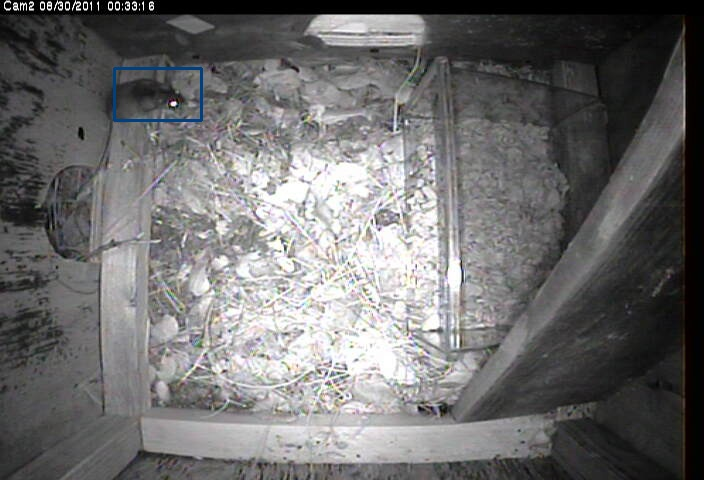
\includegraphics[width=\textwidth]{tracking.jpg}
      \vspace{5pt}
  \end{subfigure}
  \begin{subfigure}[b]{0.4\textwidth}
      \centering
      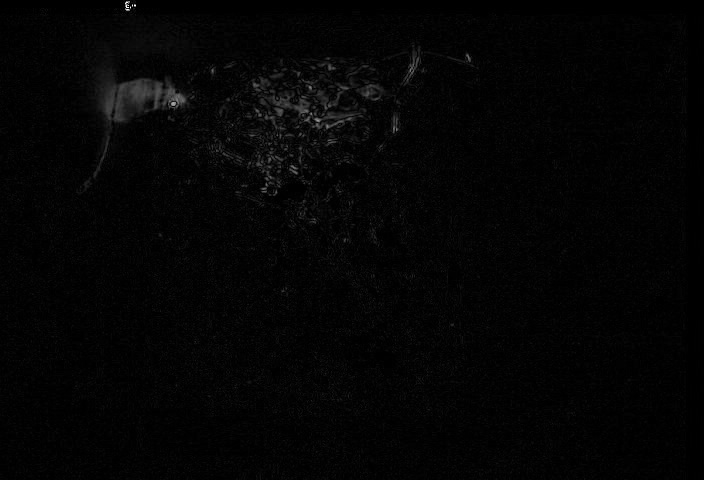
\includegraphics[width=\textwidth]{video_delta.jpg}
      \caption{delta}
  \end{subfigure} \\
  \begin{subfigure}[b]{0.4\textwidth}
      \centering
      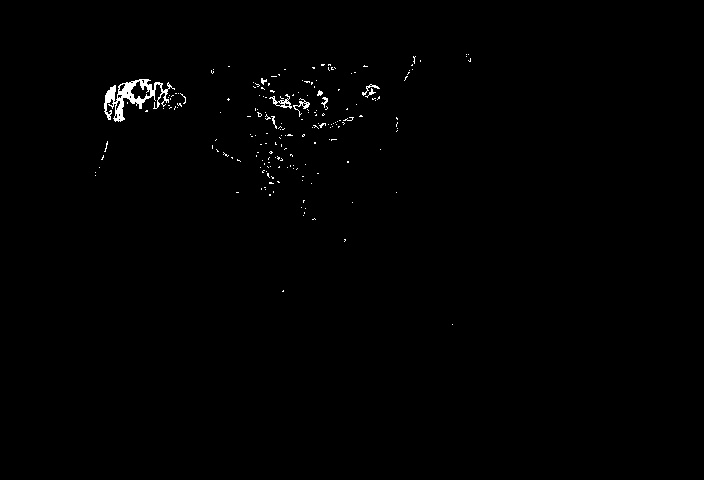
\includegraphics[width=\textwidth]{video_binthresh.jpg}
      \caption{binary threshold}
  \end{subfigure}
  \begin{subfigure}[b]{0.4\textwidth}
      \centering
      
\includegraphics[width=\textwidth]{video_binmorph.jpg}
      \caption{binary morphology}
  \end{subfigure}
  \caption{Visualisation of image processing pipeline}

\end{figure}

\end{appendices}

\end{document}
